%%%%%%%%%%%%%%%%%%%%%%%%%%%%%%%%%
% baposter Landscape Poster
% LaTeX Template
% Version 1.0 (15/5/13)
%
% Created by:
% Brian Amberg (baposter@brian-amberg.de)
%
% This template has been downloaded from:
% http://www.LaTeXTemplates.com
%
% License:
% CC BY-NC-SA 3.0 (http://creativecommons.org/licenses/by-nc-sa/3.0/)
%
%%%%%%%%%%%%%%%%%%%%%%%%%%%%%%%%%%%%%%%%%

%----------------------------------------------------------------------------------------
%	PACKAGES AND OTHER DOCUMENT CONFIGURATIONS
%----------------------------------------------------------------------------------------

\documentclass[a0paper,portrait,fontscale=0.355, margin=2cm]{baposter}

\usepackage[utf8]{inputenc}
\usepackage[font=normalsize,labelfont=bf]{caption} % Required for specifying captions to tables and figures
\captionsetup{justification=centering}
\usepackage{booktabs} % Horizontal rules in tables
\usepackage{lmodern}
\usepackage{relsize} % Used for making text smaller in some places

% Other packages
\usepackage{tabularx}
\def\tabularxcolumn#1{m{#1}}
\def\imagetop#1{\vtop{\null\hbox{#1}}}
\usepackage{adjustbox}
\usepackage{subfig}
\usepackage{floatrow} % sidecapfloat
\usepackage{setspace}
\usepackage{xspace}
\usepackage{noReferences}
\usepackage{caption}
\usepackage{tikz}
\usepackage[customcolors]{hf-tikz}
%\usepackage{subcaption}
\usepackage{epsf}
\usepackage{amsmath}
\usepackage{mathtools}
\usepackage{amssymb}
\usepackage{amsfonts}
\usepackage{amsthm}
\usepackage{dsfont}
\usepackage{enumitem}
\usepackage{float}
\usepackage{cases}
\usepackage{verbatim}
\usepackage{array}
\usepackage{graphicx}
\usepackage{graphics}
\usepackage{multirow}
\usepackage{listings}
%\usepackage[authoryear]{natbib}
\usepackage{authblk}
\usepackage[linesnumbered,ruled,vlined]{algorithm2e}
\usepackage{eqparbox}
\usepackage{xcolor}
\usepackage[backend=biber, citestyle=authoryear, maxcitenames=2, maxbibnames=2]{biblatex}
\usepackage{lipsum}
\usepackage{svg}
\usepackage{cleveref}

\bibliography{../budgeted_rl.bib}


% Arrows
\newcommand{\incarrow}{{
\includegraphics[height=0.7\baselineskip]{./img/arrow_list}}}
\newcommand{\xmark}{\ding{55}}%


% Colors for slides
\definecolor{rouge1}{RGB}{226,0,38}  % red P
\definecolor{orange1}{RGB}{243,154,38}  % orange P
\definecolor{jaune}{RGB}{254,205,27}  % jaune P
\definecolor{blanc}{RGB}{255,255,255} % blanc P

\definecolor{rouge2}{RGB}{230,68,57}  % red S
\definecolor{orange2}{RGB}{236,117,40}  % orange S
\definecolor{taupe}{RGB}{134,113,127} % taupe S
\definecolor{gris}{RGB}{91,94,111} % gris S
\definecolor{bleu1}{RGB}{38,109,131} % bleu S
\definecolor{bleu2}{RGB}{28,50,114} % bleu S
\definecolor{vert1}{RGB}{133,146,66} % vert S
\definecolor{vert3}{RGB}{20,200,66} % vert S
\definecolor{vert2}{RGB}{157,193,7} % vert S
\definecolor{vertsolarized}{RGB}{211,233,219} % vert S
\definecolor{darkyellow}{RGB}{233,165,0}  % orange S
\definecolor{lightgray}{rgb}{0.9,0.9,0.9}
\definecolor{darkgray}{rgb}{0.6,0.6,0.6}

% Highlights for slides
\newcommand{\rcol}[1]{\textcolor{red}{\textit{#1}}}
%\newcommand{\eqrcol}[1]{\textcolor{red}{#1}}
%\newcommand{\eqrcolb}[1]{\textcolor{red}{\boldsymbol{#1}}}
\newcommand{\gcol}[1]{\textcolor{vert3}{\textit{#1}}}
%\newcommand{\eqgcol}[1]{\textcolor{vert3}{#1}}
%\newcommand{\eqgcolb}[1]{\textcolor{vert3}{\boldsymbol{#1}}}
\newcommand{\blcol}[1]{\textcolor{blue}{\textit{#1}}}
%\newcommand{\eqbcol}[1]{\textcolor{blue}{#1}}
%\newcommand{\eqbcolb}[1]{\textcolor{blue}{\boldsymbol{#1}}}
\newcommand{\ycol}[1]{\textcolor{darkyellow}{\textit{#1}}}
\newcommand{\eqycol}[1]{\textcolor{darkyellow}{#1}}

\newcommand{\rcolbm}[1]{$\textcolor{red}{\boldsymbol{#1}}$}
\newcommand{\rcolb}[1]{\textcolor{red}{\textit{\textbf{#1}}}}
\newcommand{\gcolb}[1]{\textcolor{vert3}{\textit{\textbf{#1}}}}
\newcommand{\bcolb}[1]{\textcolor{blue}{\textit{\textbf{#1}}}}
\newcommand{\ycolb}[1]{\textcolor{darkyellow}{\textit{\textbf{#1}}}}

% Colored boxes
\newcounter{ColoredBoxesCounter}
\newcommand{\highlightnew}[3][(0.0,-0.1)(-0.0,0.3)]{
\hfsetfillcolor{#2!20}
\hfsetbordercolor{#2!80}
\tikzmarkin{\theColoredBoxesCounter}#1
#3
\tikzmarkend{\theColoredBoxesCounter}
\stepcounter{ColoredBoxesCounter}
}

\newcommand{\highlight}[2][yellow]{\mathchoice%
{\colorbox{#1}{$\displaystyle#2$}}%
{\colorbox{#1}{$\textstyle#2$}}%
{\colorbox{#1}{$\scriptstyle#2$}}%
{\colorbox{#1}{$\scriptscriptstyle#2$}}}%

\newcommand{\eqrcol}[1]{\highlight[red!20]{#1}}
\newcommand{\eqrcolb}[1]{\highlight[red!20]{\boldsymbol{#1}}}
\newcommand{\eqgcol}[1]{\highlight[vert3!20]{#1}}
\newcommand{\eqgcolb}[1]{\highlight[vert3!20]{\boldsymbol{#1}}}
\newcommand{\eqbcol}[1]{\highlight[blue!20]{#1}}
\newcommand{\eqbcolb}[1]{\highlight[blue!20]{\boldsymbol{#1}}}

\colorlet{redp}{red!20} % vert S
\colorlet{greenp}{vert3!20} % vert S
\colorlet{bluep}{blue!20} % vert S
\colorlet{yellowp}{yellow!20} % vert S

\newcommand{\hl}[3][\fboxsep1pt]{{#1\colorbox{#2}{#3}}}%

\newcommand{\hlr}[1]{\hl{redp}{#1}}
\newcommand{\hlg}[1]{\hl{greenp}{#1}}
\newcommand{\hlb}[1]{\hl{bluep}{#1}}
\newcommand{\hly}[1]{\hl{yellowp}{#1}}

\newcommand{\hler}[1]{\hl[\fboxsep0pt]{redp}{$\displaystyle {#1}$}}
\newcommand{\hleg}[1]{\hl[\fboxsep0pt]{greenp}{$\displaystyle {#1}$}}
\newcommand{\hleb}[1]{\hl[\fboxsep0pt]{bluep}{$\displaystyle {#1}$}}

\newcommand{\hlbr}[1]{\hl[\fboxsep0pt]{redp}{$\displaystyle \mathbf{#1}$}}
\newcommand{\hlbg}[1]{\hl[\fboxsep0pt]{greenp}{$\displaystyle \mathbf{#1}$}}
\newcommand{\hlbb}[1]{\hl[\fboxsep0pt]{bluep}{$\displaystyle \mathbf{#1}$}}

\newcommand{\vph}{\vphantom{A_A^A}}

% Box for algorithms
\newlength{\minipagewidth}
\newlength{\minipagewidthx}
\setlength{\minipagewidth}{\columnwidth}
\setlength{\minipagewidthx}{\columnwidth}
\setlength{\fboxsep}{0.1mm}
\addtolength{\minipagewidth}{-\fboxrule}
\addtolength{\minipagewidth}{-\fboxrule}
\addtolength{\minipagewidth}{-\fboxsep}
\addtolength{\minipagewidth}{-\fboxsep}
\addtolength{\minipagewidthx}{+\fboxsep}
\newcommand{\bookbox}[1]{\small
\par\medskip\noindent
\framebox[\columnwidth]{
\begin{minipage}{\minipagewidth} {#1} \end{minipage} } \par\medskip }

\newcommand{\bookboxx}[1]{
\par\medskip\noindent
\framebox[\columnwidth]{
\begin{minipage}[t]{0.98\columnwidth} {\par\smallskip#1\par\smallskip} \end{minipage} } \par\medskip }


\usepackage{array}
\newcolumntype{L}[1]{>{\raggedright\let\newline\\\arraybackslash\hspace{-3.1cm}}m{#1}}
\newcolumntype{C}[1]{>{\centering\let\newline\\\arraybackslash\hspace{135pt}}m{#1}}
\newcolumntype{R}[1]{>{\raggedleft\let\newline\\\arraybackslash\hspace{-10pt}}m{#1}}

\newenvironment{myfont}{\fontfamily{kurier}\selectfont}{\par}
\newenvironment{myfont2}{\fontfamily{epigrafica}\selectfont}{\par}

% Border color of content boxes
\definecolor{bordercol}{RGB}{0,0,0}  %black
% Background color for the header in the content boxes (left side)
\definecolor{headercol1}{RGB}{200,0,0}        %red:RGB {200,0,0} 
% Background color for the header in the content boxes (right side) 
\definecolor{headercol2}{rgb}{1.0,0.49,0.0}        %orange:rgb {1.0,0.49,0.0}
% Text color for the header text in the content boxes
\definecolor{headerfontcol}{rgb}{1,1,1}  %white
% Background color for the content in the boxes
\definecolor{boxcolor}{rgb}{1,1,1} 

\definecolor{lightblue}{rgb}{0.145,0.6666,1}

\newsavebox\CBox
\newcommand\hcancel[2][0.5pt]{%
  \ifmmode\sbox\CBox{$#2$}\else\sbox\CBox{#2}\fi%
  \makebox[0pt][l]{\usebox\CBox}%  
  \rule[0.3\ht\CBox-#1/2]{\wd\CBox}{#1}}



%%%%%%%%%%%%%%%%%%%%%%%%%%%%
% Paper dependent stuff    %
%%%%%%%%%%%%%%%%%%%%%%%%%%%%

\newcommand{\FTQ}{\textcolor{myalgocolor}{\normalfont \texttt{FTQ}}\xspace}
\newcommand{\FTQl}{\textcolor{myalgocolor}{\normalfont \texttt{FTQ}$(\lambda)$}\xspace}
\newcommand{\BFTQ}{\textcolor{myalgocolor}{\normalfont \texttt{BFTQ}}\xspace}
\newcommand{\ov}{\overline}
\newcommand{\oa}{\ov{a}}
\newcommand{\ox}{\ov{x}}
\newcommand{\oz}{\ov{z}}
\newcommand{\oy}{\ov{y}}
\newcommand{\os}{\ov{s}}
\newcommand{\ocS}{\ov{\cS}}
\newcommand{\ocA}{\ov{\cA}}

%%%%%%%%%%%%%%%%%%%%%%%%%%%%
% Aesthetics               %
% over-underline, hat, bold%
%%%%%%%%%%%%%%%%%%%%%%%%%%%%

\newcommand{\eps}{\varepsilon}
\newcommand{\vareps}{\varepsilon}
\renewcommand{\epsilon}{\varepsilon}
%\renewcommand{\hat}{\widehat}
\renewcommand{\tilde}{\widetilde}
\renewcommand{\bar}{\overline}

\newcommand*{\MyDef}{\mathrm{\tiny def}}
\newcommand*{\eqdefU}{\ensuremath{\mathop{\overset{\MyDef}{=}}}}% Unscaled version
\newcommand*{\eqdef}{\mathop{\overset{\MyDef}{\resizebox{\widthof{\eqdefU}}{\heightof{=}}{=}}}}


\def\:#1{\protect \ifmmode {\mathbf{#1}} \else {\textbf{#1}} \fi}
\newcommand{\CommaBin}{\mathbin{\raisebox{0.5ex}{,}}}

\newcommand{\wt}[1]{\widetilde{#1}}
\newcommand{\wh}[1]{\widehat{#1}}
\newcommand{\wo}[1]{\overline{#1}}
\newcommand{\wb}[1]{\overline{#1}}

% bf and bm missing due to conflict!!
\newcommand{\bsym}[1]{\mathbf{#1}}
\newcommand{\bzero}{\mathbf{0}}
\newcommand{\ba}{\mathbf{a}}
\newcommand{\bb}{\mathbf{b}}
\newcommand{\bc}{\mathbf{c}}
\newcommand{\bd}{\mathbf{d}}
\newcommand{\be}{\mathbf{e}}
\newcommand{\bbE}{\mathbb{E}}
\newcommand{\bg}{\mathbf{g}}
\newcommand{\bh}{\mathbf{h}}
\newcommand{\bi}{\mathbf{i}}
\newcommand{\bj}{\mathbf{j}}
\newcommand{\bk}{\mathbf{k}}
\newcommand{\bl}{\mathbf{l}}
\newcommand{\bn}{\mathbf{n}}
\newcommand{\bo}{\mathbf{o}}
\newcommand{\bp}{\mathbf{p}}
\newcommand{\bq}{\mathbf{q}}
\newcommand{\br}{\mathbf{r}}
\newcommand{\bs}{\mathbf{s}}
\newcommand{\bt}{\mathbf{t}}
\newcommand{\bu}{\mathbf{u}}
\newcommand{\bv}{\mathbf{v}}
\newcommand{\bw}{\mathbf{w}}
\newcommand{\bx}{\mathbf{x}}
\newcommand{\by}{\mathbf{y}}
\newcommand{\bz}{\mathbf{z}}

\newcommand{\bA}{\mathbf{A}}
\newcommand{\bB}{\mathbf{B}}
\newcommand{\bC}{\mathbf{C}}
\newcommand{\bD}{\mathbf{D}}
\newcommand{\bE}{\mathbf{E}}
\newcommand{\bF}{\mathbf{F}}
\newcommand{\bG}{\mathbf{G}}
\newcommand{\bH}{\mathbf{H}}
\newcommand{\bI}{\mathbf{I}}
\newcommand{\bJ}{\mathbf{J}}
\newcommand{\bK}{\mathbf{K}}
\newcommand{\bL}{\mathbf{L}}
\newcommand{\bM}{\mathbf{M}}
\newcommand{\bN}{\mathbf{N}}
\newcommand{\bO}{\mathbf{O}}
\newcommand{\bP}{\mathbf{P}}
\newcommand{\bQ}{\mathbf{Q}}
\newcommand{\bR}{\mathbf{R}}
\newcommand{\bS}{\mathbf{S}}
\newcommand{\bT}{\mathbf{T}}
\newcommand{\bU}{\mathbf{U}}
\newcommand{\bV}{\mathbf{V}}
\newcommand{\bW}{\mathbf{W}}
\newcommand{\bX}{\mathbf{X}}
\newcommand{\bY}{\mathbf{Y}}
\newcommand{\bZ}{\mathbf{Z}}

% calligraphic
\newcommand{\cf}{\mathcal{f}}
\newcommand{\cA}{\mathcal{A}}
\newcommand{\cB}{\mathcal{B}}
\newcommand{\cC}{\mathcal{C}}
\newcommand{\cD}{\mathcal{D}}
\newcommand{\cE}{\mathcal{E}}
\newcommand{\cF}{\mathcal{F}}
\newcommand{\cG}{\mathcal{G}}
\newcommand{\cH}{\mathcal{H}}
\newcommand{\cI}{\mathcal{I}}
\newcommand{\cJ}{\mathcal{J}}
\newcommand{\cK}{\mathcal{K}}
\newcommand{\cL}{\mathcal{L}}
\newcommand{\cM}{\mathcal{M}}
\newcommand{\cN}{\mathcal{N}}
\newcommand{\cO}{\mathcal{O}}
\newcommand{\cP}{\mathcal{P}}
\newcommand{\cQ}{\mathcal{Q}}
\newcommand{\cR}{\mathcal{R}}
\newcommand{\cS}{\mathcal{S}}
\newcommand{\cT}{\mathcal{T}}
\newcommand{\cU}{\mathcal{U}}
\newcommand{\cV}{\mathcal{V}}
\newcommand{\cW}{\mathcal{W}}
\newcommand{\cX}{\mathcal{X}}
\newcommand{\cY}{\mathcal{Y}}
\newcommand{\cZ}{\mathcal{Z}}

%%%%%%%%%%%%%%%%%%%%%%%%%%%%
% Math jargon              %
%%%%%%%%%%%%%%%%%%%%%%%%%%%%
\newcommand{\wrt}{w.r.t.\xspace}
\newcommand{\defeq}{\stackrel{\mathclap{\normalfont\mbox{\tiny def}}}{=}}
\newcommand{\maxund}[1]{\max\limits_{#1}}
\newcommand{\supund}[1]{\text{sup}\limits_{#1}}
\newcommand{\minund}[1]{\min\limits_{#1}}
\renewcommand{\epsilon}{\varepsilon}
\newcommand{\bigotime}{\mathcal{O}}


\DeclareMathOperator*{\argmin}{arg\,min}
\DeclareMathOperator*{\argmax}{arg\,max}
\DeclareMathOperator*{\cupdot}{\mathbin{\mathaccent\cdot\cup}}

%%%%%%%%%%%%%%%%%%%%%%%%%%%%
% Matrix operators         %
%%%%%%%%%%%%%%%%%%%%%%%%%%%%
\newcommand{\transpose}{^\mathsf{\scriptscriptstyle T}}
\newcommand{\transp}{\mathsf{\scriptscriptstyle T}}

%%%%%%%%%%%%%%%%%%%%%%%%%%%%
% Statistic operators      %
%%%%%%%%%%%%%%%%%%%%%%%%%%%%
\newcommand{\probability}[1]{\mathbb{P}\left(#1\right)}
\newcommand{\probdist}{Pr}
\DeclareMathOperator*{\expectedvalue}{\mathbb{E}}
\DeclareMathOperator*{\variance}{\text{Var}}
\newcommand{\expectedvalueover}[1]{\expectedvalue\limits_{#1}}
\newcommand{\condbar}{\;\middle|\;}
\newcommand{\gaussdistr}{\mathcal{N}}
\newcommand{\uniformdistr}{\mathcal{U}}
\newcommand{\bernoullidist}{\mathcal{B}}

%%%%%%%%%%%%%%%%%%%%%%%%%%%%
% Algebraic Sets           %
%%%%%%%%%%%%%%%%%%%%%%%%%%%%
\newcommand{\Real}{\mathbb{R}}
\newcommand{\Natural}{\mathbb{N}}
\newcommand{\statespace}{\mathcal{X}}
\newcommand{\funcspace}{\mathcal{F}}
\newcommand{\dynaspace}{\mathcal{T}}

%
%\newtheorem{theorem}{Theorem}
%\newtheorem{definition}{Definition}
%\newtheorem{lemma}{Lemma}
\newtheorem{proposition}{Proposition}
\newtheorem{remark}{Remark}
\newtheorem{conjecture}{Conjecture}
%\newtheorem{property}{Property}
%\newtheorem{assumption}{Assumption}
%\newtheorem{conjecture}{Conjecture}
%
%\newtheorem*{definition*}{Definition}
%\newtheorem*{theorem*}{Theorem}
%\newtheorem*{proposition*}{Proposition}
%\newtheorem*{remark*}{Remark}


\begin{document}


%\background{ % Set the background to an image (background.pdf)
%\begin{tikzpicture}[remember picture,overlay]
%\draw (current page.north west)+(-2em,2em) node[anchor=north west]
%{\includegraphics[height=1.1\textheight]{background.png}};
%\end{tikzpicture}
%}
\begin{poster}{
grid=false,
borderColor=bordercol, % Border color of content boxes
headerColorOne=headercol1, % Background color for the header in the content boxes (left side)
headerColorTwo=headercol2, % Background color for the header in the content boxes (right side)
headerFontColor=headerfontcol, % Text color for the header text in the content boxes
boxColorOne=boxcolor, % Background color for the content in the content boxes
headershape=roundedright, % Specify the rounded corner in the content box headers
%headerfont=\Large\sf\bf, % Font modifiers for the text in the content box headers
headerfont=\Large\bf\textsc, %Sans Serif
textborder=rectangle,
background=none,
headerborder=open, % Change to closed for a line under the content box headers
boxshade=plain,
textfont={\setlength{\parindent}{0.0em}\sffamily},
headerheight={0.05\textheight},
eyecatcher=true
%columns=5
}
%
%----------------------------------------------------------------------------------------
%	Title and authors
%----------------------------------------------------------------------------------------
%
{

\includegraphics[width=18em]{./img/companies}
}
{
Budgeted Reinforcement Learning in Continuous State Space
}
{
Nicolas Carrara, Edouard Leurent, Romain Laroche, \\Tanguy Urvoy, Odalric-Ambrym Maillard, Olivier Pietquin
\vspace{-3\baselineskip}
}
{

\includegraphics[width=14em]{./img/inria_sc}
}

\setlength{\colheight}{0.92\textheight}

%----------------------------------------------------------------------------------------
%	Motivation
%----------------------------------------------------------------------------------------

\headerbox{\textsc{Motivation}}{name=motivation,span=1,column=0,row=0}{

\textbf{Markov Decision Process} $(\cS, \cA, P, R_r, \gamma)$:
\begin{equation*}
    \max_\pi \expectedvalue_\pi \underbrace{\sum_{t=0}^\infty \gamma^t R_r(s_t, a_t)}_{G_r^\pi}
\end{equation*}

\begin{itemize}[nolistsep]
    \item[\incarrow] \hlr{Single scalar reward} to represent \hlr{multiple} \hlr{contradictory} aspects (e.g. complete task and avoid collisions)
    \item[\incarrow] \hlr{No control over the spread} of the performance distribution\\
     
\end{itemize}

\textbf{Constrained MDP} $(\cS, \cA, P, R_r, R_c, \gamma)$
\begin{itemize}[nolistsep]
    \item $[$\cite{BEUTLER1985236,Altman95constrainedmarkov}$]$
    \item Introduce a \hlb{cost signal} $R_c$
    \item Constrained objective
\begin{equation*}
\begin{array}{lcr}
 \displaystyle \max_{\pi\in\cM(\cA)^\cS} \expectedvalue[G_r^\pi | s_0=s] & \text{\hlb{ s.t. }} & \expectedvalue[G_c^\pi | s_0=s] \leq \beta
\end{array}
\end{equation*}
\item[\incarrow] The cost budget $\beta$ \hlr{cannot be changed} after training\\
\end{itemize}

\textbf{Budgeted MDP}

\begin{itemize}[nolistsep]
    \item $[$\cite{Boutilier_Lu:uai16}$]$
    \item We seek \hlg{one general policy} $\pi(s,\beta)$ that solves every CMDP for any $\beta$
    \item[\incarrow] Can only be solved for \hlr{finite} $\cS$ and \hlr{known} $P, R_r, R_c$.
\end{itemize}
}

%----------------------------------------------------------------------------------------
%	Setting
%----------------------------------------------------------------------------------------
\headerbox{\textsc{Setting}}{name=setting,span=1,column=0,row=0,below=motivation}{

\textbf{Budgeted policies} $\pi$
\begin{itemize}
    \item Take a budget $\beta$ as an additional input
    \item Output a next budget $\beta'$ 
\end{itemize}
\begin{equation*}
    \pi:\underbrace{(s,\beta)}_{\os} \rightarrow \underbrace{(a,\beta')}_{\oa}
\end{equation*}

\textbf{2D  signals}
\begin{enumerate}
    \item Rewards $R = (R_r, R_c)$
    \item Returns $G^\pi = (G_r^\pi, G_c^\pi)$
    \item Values $V^\pi = (V_r^\pi, V_c^\pi)$ and $Q^\pi = (Q_r^\pi, Q_c^\pi)$\\
\end{enumerate}

\textbf{Policy Evaluation}\\

The Bellman Expectation equations% [\cite{Bellman}]
are preserved, and the Bellman Expectation Operator $\cT^\pi$ is a \hlg{$\gamma$-contraction}.
}

%----------------------------------------------------------------------------------------
%	Budgeted Optimality
%----------------------------------------------------------------------------------------
\headerbox{Budgeted Optimality}{name=bopt,column=0,span=1,below=setting}{
\begin{definition*}In that order, we want to:
\begin{enumerate}
    \item[(i)] \hlb{Respect the budget $\beta$}: 
    \begin{equation*}
    \Pi_a(\os) \eqdef \{\pi\in\Pi: V_c^\pi(s, \beta) \leq \beta\}
    \end{equation*}
    \item[(ii)] \hlg{Maximise the rewards}:
    \begin{equation*}
        V_r^*(\os) \eqdef {\max}_{\pi\in\Pi_a(\os)}  V_r^\pi(\os) \qquad\quad \Pi_r(\os) \eqdef \argmax_{\pi\in\Pi_a(\os)}  V_r^\pi(\os)
    \end{equation*}
    \item[(iii)] \hlr{Minimise the costs}: 
    \begin{equation*}
        V_c^*(\os) \eqdef {\min}_{\pi\in\Pi_r(\os)}  V_c^\pi(\os), \qquad\quad \Pi^*(\os) \eqdef \argmin_{\pi\in\Pi_r(\os)}  V_c^\pi(\os)
    \end{equation*}
\end{enumerate}

We define the budgeted action-value function $Q^*$ similarly
\end{definition*}

}

%----------------------------------------------------------------------------------------
%	Budgeted Dynamic Programming
%----------------------------------------------------------------------------------------
\headerbox{Budgeted Dynamic Programming}{name=bdp,column=1,span=2}{

\begin{minipage}{0.7\textwidth}
\bookboxx{
\begin{theorem*}[Budgeted Bellman Optimality]
\label{thm:bellman-optimality}
$Q^*$ verifies:
\begin{equation}
\label{eq:bellman-optimality}
    \hleb{\vphantom{\frac{A}{A}} Q^{*}(\os, \oa) = \cT Q^{*}(\os, \oa)}  \eqdef R(\os, \oa) + \gamma \sum_{\os'\in\ocS} \ov{P}(\ov{s'} | \os, \oa)\sum_{\ov{a'}\in \ocA} \pi_\text{greedy}(\ov{a'}|\ov{s'}; Q^*) Q^{*}(\ov{s'}, \ov{a'}),
\end{equation}
where the greedy policy $\pi_\text{greedy}$ is defined by:
\begin{subequations}
\label{eq:pi_greedy}
\begin{align}
    \pi_\text{greedy}(\oa|\os; Q) \in &\hler{\argmin}_{\rho\in\Pi_r^Q} \expectedvalueover{\oa\sim\rho}Q_c(\os, \oa), \label{eq:pi_greedy_cost}\\
    \text{where }\quad\Pi_r^Q \eqdef &\hleg{\argmax}_{\rho\in\cM(\ocA)} \expectedvalueover{\oa\sim\rho} Q_r(\os, \oa) \label{eq:pi_greedy_reward}\\
    & \text{ s.t. }  \expectedvalueover{\oa\sim\rho} Q_c(\os, \oa) \hleb{\leq \beta} \label{eq:pi_greedy_constraint}
\end{align}
\end{subequations}
\end{theorem*}
}
\bookboxx{
\begin{proposition*}
\label{prop:greedy_optimal}
$\pi_\text{greedy}(\cdot~; Q^*)$ is \hlg{simultaneously optimal} in all states $\os\in\ocS$: $$\pi_\text{greedy}(\cdot~; Q^*)\in\Pi^*(\os)$$

In particular, $V^{\pi_\text{greedy}(\cdot; Q^*)} = V^*$ and $Q^{\pi_\text{greedy}(\cdot; Q^*)}= Q^*$.
\end{proposition*}
}

\end{minipage}
\hfill%
\begin{minipage}{0.25\textwidth}
\begin{algorithm}[H]
\DontPrintSemicolon
\KwData{$P, R_r, R_c$}
\KwResult{$Q^*$}
$Q_{0} \leftarrow 0$\;
\Repeat{convergence}{
    $Q_{k+1} \leftarrow \cT Q_k$\;
}
\caption{Budgeted Value Iteration}
\label{algo:bvi}
\end{algorithm}
\begin{center}
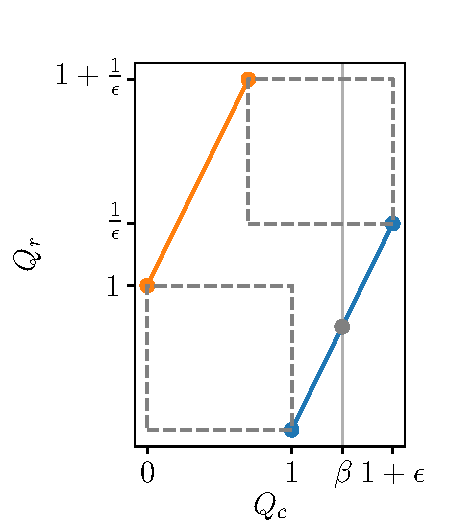
\includegraphics[width=0.9\textwidth]{source/img/concavity_example.pdf}    
\end{center}
\end{minipage}

\bookboxx{
\begin{theorem*}[Contractivity]
\label{thm:contraction}
For any BMDP ($\cS,\cA,P,R_r,R_c,\gamma$) with $|\cA| \geq 2$, \hlr{$\cT$ is not a contraction}. 
$$\forall\epsilon>0, \exists Q^1,Q^2\in(\Real^2)^{\ocS\ocA}:\|\cT Q^1-\cT Q^2\|_\infty \geq \frac{1}{\epsilon}\|Q^1-Q^2\|_\infty$$
\end{theorem*}
}

Despite those theoretical limitations, we observed \hlg{empirical convergence} in our experiments

\bookboxx{
\begin{remark*}[Contractivity on smooth $Q$-functions]
\label{rmk:contractivity-smooth}
We conjecture that \hlg{$\cT$ is a contraction when restricted} to the subset $\cL_\gamma$ of $Q$-functions such that "$Q_r$ is \hlg{$L$-Lipschitz} with respect to $Q_c$", with $L<\frac{1}{\gamma}-1$.
\end{remark*}
}
}

%----------------------------------------------------------------------------------------
%	Budgeted Reinforcement Learning
%----------------------------------------------------------------------------------------
\headerbox{Budgeted Reinforcement Learning}
{name=brl,span=2,column=1,below=bdp}{ 

We address several limitations of \Cref{algo:bvi}.\\

\begin{minipage}{0.65\textwidth}
\begin{enumerate}
    \item The BMDP is \hlr{unknown}
\begin{itemize}[nolistsep]
    \item[\incarrow] Work with a \hlg{batch} of samples $\cD=\{(\os_i,\oa_i,r_i,\os_i'\}_{i\in [0,N]}$
\end{itemize}
\item $\cT$ contains an \hlr{expectation} $\expectedvalue_{\os'\sim \ov{P}}$ over next states $\os'$
\begin{itemize}[nolistsep]
    \item[\incarrow] Replace it with a \hlg{sampling} operator $\hat{\cT}$:
\begin{equation*}
    \hat{\cT} Q(\os_i, \oa_i, r_i, \os'_i) \eqdef r_i + \gamma \sum_{\ov{a'_i}\in \cA_i} \pi_\text{greedy}(\ov{a'_i}|\ov{s'_i}; Q) Q(\ov{s'_i}, \ov{a'_i}).
\end{equation*}
\end{itemize}
\item $\cS$ is \hlr{continuous}
\begin{itemize}[nolistsep]
    \item[\incarrow] Employ \hlg{function approximation} $Q_\theta$, and minimise a regression loss 
    $$\cL(Q_\theta, Q_\text{target};\cD) = \sum_{\cD} ||Q_\theta(\os, \oa) - Q_\text{target}(\os, \oa, r, \os')||_2^2$$
\end{itemize}
\end{enumerate}

\end{minipage}
\begin{minipage}{0.34\textwidth}
\begin{algorithm}[H]
\DontPrintSemicolon
\KwData{$\cD$}
\KwResult{$Q^*$}
$Q_{\theta_0} \leftarrow 0$\;
\Repeat{convergence}{
    $\theta_{k+1} \leftarrow \argmin_\theta \cL(Q_\theta, \hat{\cT} Q_{\theta_{k}}; \cD)$\;
}
\caption{Budgeted Fitted-Q Iteration}
\label{algo:bftq}
\end{algorithm}
\vspace{1em}
\begin{enumerate}[nolistsep]
    \item[4.] How to \hlr{collect the batch} $\cD$?
    \begin{itemize}[nolistsep]
        \item[\incarrow] We propose a \hlg{risk-sensitive} exploration procedure
    \end{itemize}
\end{enumerate}
\end{minipage}
}

%----------------------------------------------------------------------------------------
%	Scalable Implementation
%----------------------------------------------------------------------------------------
\headerbox{Scalable Implementation}{name=scale,span=2,column=1,below=brl}{ 

\begin{minipage}[t]{0.48\textwidth}
\textbf{How to compute the greedy policy?}

\begin{center}
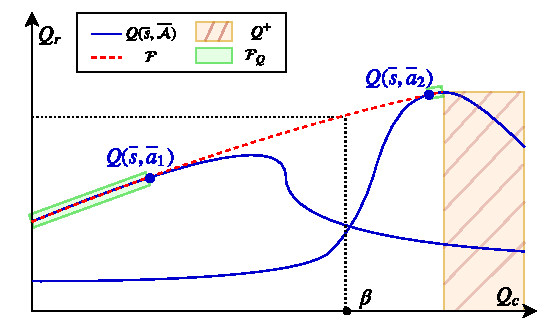
\includegraphics[width=0.8\linewidth]{../source/img/pi.pdf}    
\end{center}
\vspace*{-1em}
\bookboxx{
\begin{proposition*}[Hull policy]
\label{prop:bftq_pi_hull}
$\pi_\text{greedy}$ in \eqref{eq:pi_greedy} can be \hlg{computed explicitly}, as a mixture of two points that lie on the convex hull of $Q$.
\end{proposition*}
}

\end{minipage}
\hfill%
\begin{minipage}[t]{0.48\textwidth}

\textbf{Function approximation}

\begin{center}
\resizebox{.7\textwidth}{!}{%

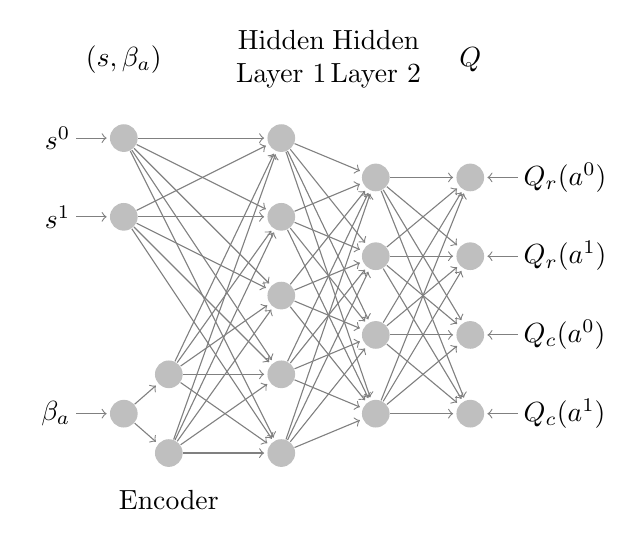
\begin{tikzpicture}[shorten >=1pt,->,draw=black!50, inner sep=1pt, node distance=\layersep]
        \tikzstyle{every pin edge}=[<-,shorten <=1pt]
        \tikzstyle{neuron}=[circle,fill=black!25,minimum size=10pt,inner sep=0pt]
        \tikzstyle{input neuron}=[neuron];
        \tikzstyle{input beta}=[neuron];
        \tikzstyle{qc}=[neuron];
        \tikzstyle{qr}=[neuron];
        \tikzstyle{hidden neuron}=[neuron];
        \tikzstyle{autoencoder neuron}=[neuron];
        \tikzstyle{annot} = [text width=4em, text centered]
        \tikzstyle{annot2} = [text width=10em, text centered]
        \def\layersep{2cm}
        % Draw the input layer nodes
        \foreach \name / \y in {0,...,1}
            \pgfmathtruncatemacro{\y}{0 + \y}
            \node[input neuron, pin=left:$s^\y$] (I-\name) at (0,-\y) {};

         % first layer
        \foreach \name / \y in {0,...,4}
        \pgfmathtruncatemacro{\y}{0 + \y}
            \path node[hidden neuron] (H1-\name) at (1*\layersep,-\y cm) {};

        \foreach \source in {0,...,1}
            \foreach \dest in {0,...,4}
                \path (I-\source) edge (H1-\dest);

        % BETA
        \node[input beta, pin=left:$\beta_a$] (BETA) at (0,-3.5) {};

        % beta auto encoder
        \foreach \name / \y in {0,...,1}
            \pgfmathtruncatemacro{\ybis}{3+ \y}
            \path node[autoencoder neuron] (AE-\name) at (\layersep/3.5,-\ybis cm) {};



        \foreach \name / \y in {0,...,3}
        \pgfmathtruncatemacro{\y}{0 + \y}
            \path[yshift=-0.5cm]
            node[hidden neuron] (H2-\name) at (1.6*\layersep,-\y cm) {};


        % actions
        \foreach \name / \y in {0,...,1}
        \pgfmathtruncatemacro{\y}{0 + \y}
            \path[yshift=-0.5cm] node[qr,pin=right:$Q_r(a^\y)$] (Qr-\name) at (2.2*\layersep,-\y cm) {};

        \foreach \name / \y in {0,...,1}
        \pgfmathtruncatemacro{\yy}{2 + \y}
            \path[yshift=-0.5cm] node[qc,pin=right:$Q_c(a^\y)$] (Qc-\name) at (2.2*\layersep,-\yy cm) {};

        \foreach \source in {0,...,1}
            \foreach \dest in {0,...,4}
                \path (AE-\source) edge (H1-\dest);



        \foreach \dest in {0,...,1}
            \path (BETA) edge (AE-\dest);

         \foreach \source in {0,...,4}
            \foreach \dest in {0,...,3}
                \path (H1-\source) edge (H2-\dest);

        \foreach \source in {0,...,3}
            \foreach \dest in {0,...,1}
                \path (H2-\source) edge (Qr-\dest);

         \foreach \source in {0,...,3}
            \foreach \dest in {0,...,1}
                \path (H2-\source) edge (Qc-\dest);
        % Annotate the layers
       \node[annot] (input) at (0,1) {$(s,\beta_a)$};
       \node[annot2] (input) at (\layersep/3.5,-4.6) {Encoder};
       \node[annot](h1) at (\layersep,1) {Hidden Layer 1};
       \node[annot](h2) at(1.6* \layersep,1) {Hidden Layer 2};
       \node[annot](output) at(2.2* \layersep,1) {$Q$};
        %\node[annot,right of=hl] {Output layer};
    \end{tikzpicture}

}    
\end{center}


\textbf{Parallel computing}

Experience collection and computation of $\pi_\text{greedy}$ can be distributed over several cores.

\end{minipage}
}

%
%%----------------------------------------------------------------------------------------
%% Experiments
%%----------------------------------------------------------------------------------------
%
\headerbox{Experiments}{name=experiments,span=2,column=1,below=scale, above=bottom}{ 

\begin{minipage}{0.49\textwidth}
\centering
Risk-sensitive exploration

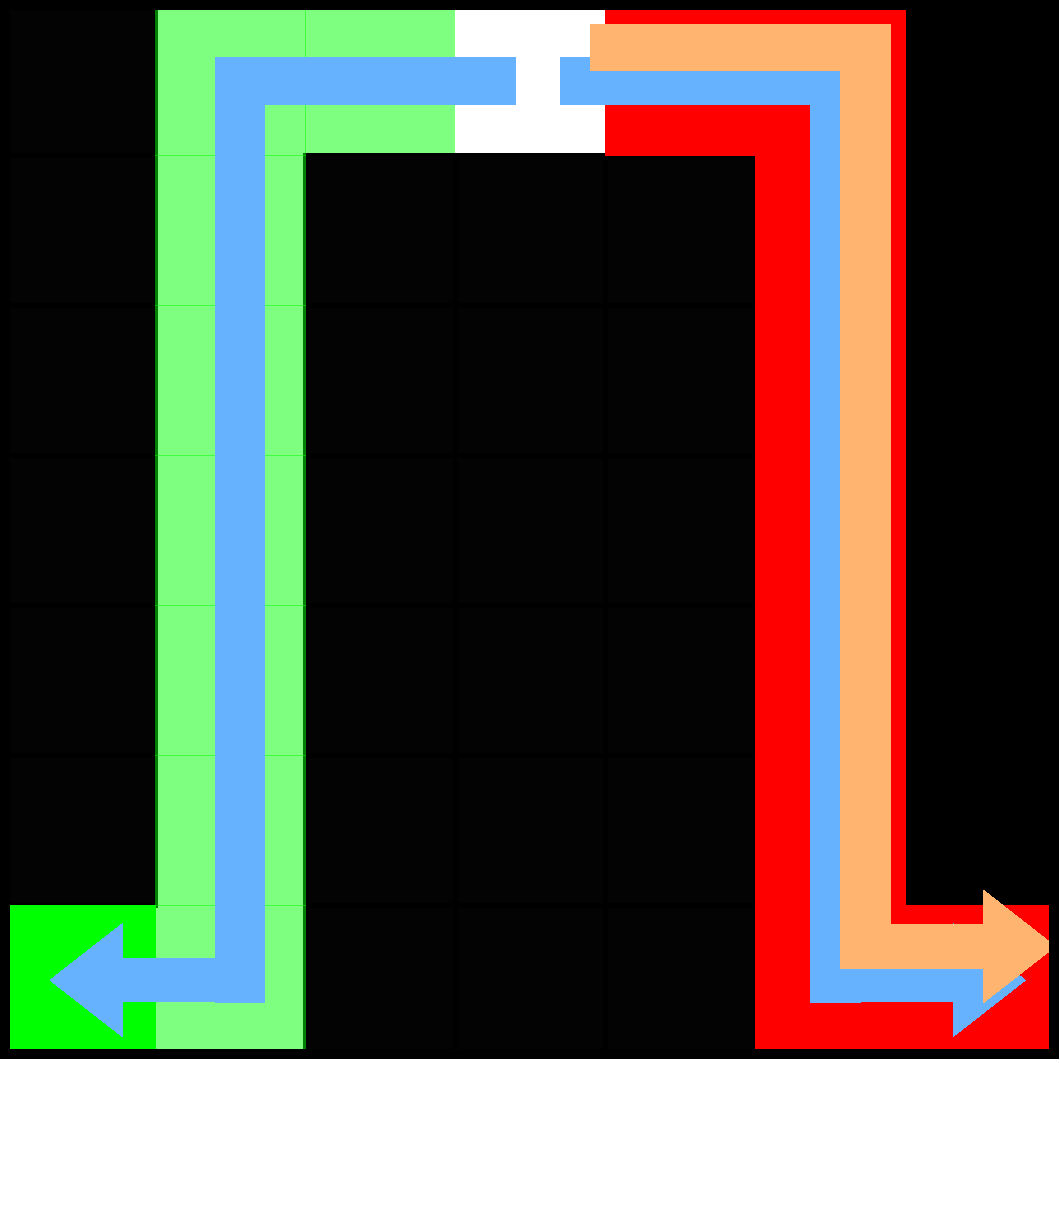
\includegraphics[width=0.3\textwidth]{source/img/test.pdf}
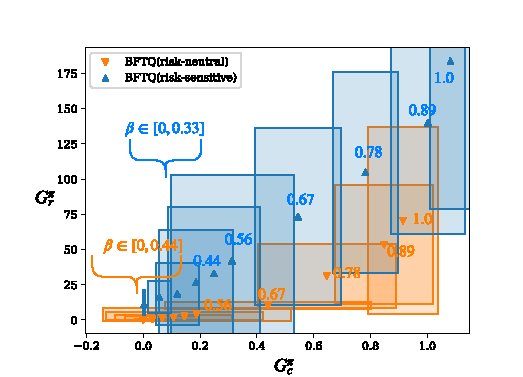
\includegraphics[page=1, width=0.49\textwidth]{source/img/corridors}
\end{minipage}
\begin{minipage}{0.5\textwidth}
\centering
Pareto frontier

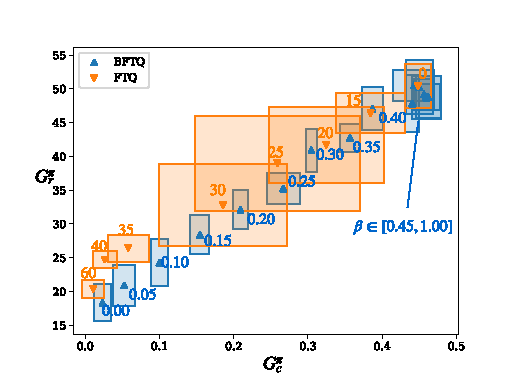
\includegraphics[width=0.49\linewidth]{../source/img/slot-filling}
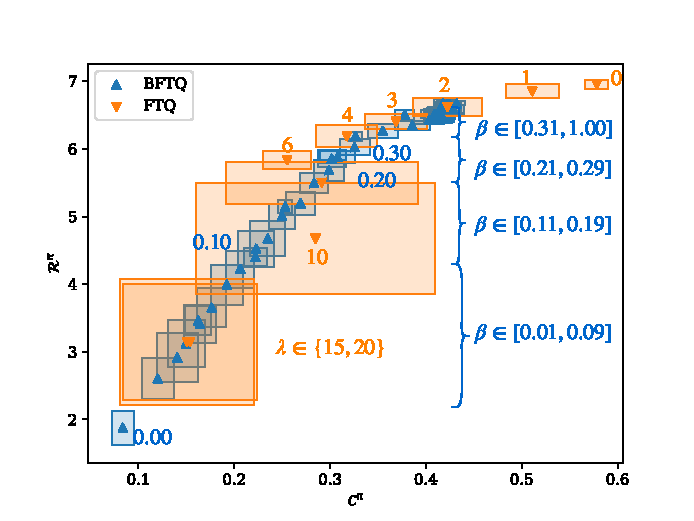
\includegraphics[width=0.49\linewidth]{../source/img/highway}
\end{minipage}
}



%----------------------------------------------------------------------------------------
%	Acknowledgements
%----------------------------------------------------------------------------------------
\headerbox{Acknowledgements}{name=ack,column=0,span=1,below=bopt}{
This work has been supported by CPER Nord-Pas de Calais/FEDER DATA Advanced data science and technologies 2015-2020, the French Ministry of Higher Education and Research, INRIA, and the French Agence Nationale de la Recherche (ANR).
}


%----------------------------------------------------------------------------------------
%	References
%----------------------------------------------------------------------------------------
\headerbox{References}{name=refs,column=0,span=1,below=ack, above=bottom}{
    {
    \AtNextBibliography{\footnotesize}
    \setlength{\bibitemsep}{3pt}
    \printbibliography[heading=none]
    }
}


\end{poster}

\end{document}


